\documentclass[paper=a4, fontsize=13pt]{extarticle} % A4 paper and 11pt font size
\usepackage{longtable} % Allows tables to span multiple pages (this package must be called before hyperref)
\usepackage{natbib}
\bibliographystyle{chicago}
\renewcommand{\familydefault}{\rmdefault}
\usepackage{lmodern}
\usepackage[T1]{fontenc} % Use 8-bit encoding that has 256 glyphs
\usepackage{fourier} % Use the Adobe Utopia font for the document - comment this line to return to the LaTeX default
\usepackage[english]{babel} % English language/hyphenation
\usepackage{amsmath,amsfonts,amsthm,tikz} % Math packages
\usepackage{multicol}
\usepackage{graphicx}
\usepackage{lipsum} % Used for inserting dummy 'Lorem ipsum' text into the template
\usepackage{subfigure}
\usepackage{here}
\usepackage{setspace}
\usepackage{amssymb}
\usepackage{wasysym}
\usepackage[center]{caption}
\usepackage[hidelinks]{hyperref}

\usepackage{multirow}

\usepackage{array}
\newcolumntype{L}[1]{>{\raggedright\let\newline\\\arraybackslash\hspace{0pt}}m{#1}}
\newcolumntype{C}[1]{>{\centering\let\newline\\\arraybackslash\hspace{0pt}}m{#1}}
\newcolumntype{R}[1]{>{\raggedleft\let\newline\\\arraybackslash\hspace{0pt}}m{#1}}

\usepackage{xcolor}
\hypersetup{
    colorlinks,
    linkcolor={red!50!black},
    citecolor={blue!50!black},
    urlcolor={blue!80!black}
}
\newcommand\independent{\protect\mathpalette{\protect\independenT}{\perp}}
\def\independenT#1#2{\mathrel{\rlap{$#1#2$}\mkern2mu{#1#2}}}
\newtheorem{proposition}{Proposition}
\newtheorem{mydef}{Definition}
\newtheorem{lemma}{Lemma}
\newtheorem{thm}{Theorem}
\newtheorem{corollary}{Corollary}
\newtheorem{ass}{Assumption}
\newtheorem{nota}{Notation}
\usepackage{fullpage}
\onehalfspacing
\allowdisplaybreaks

\numberwithin{equation}{section} % Number equations within sections (i.e. 1.1, 1.2, 2.1, 2.2 instead of 1, 2, 3, 4)
\numberwithin{figure}{section} % Number figures within sections (i.e. 1.1, 1.2, 2.1, 2.2 instead of 1, 2, 3, 4)
\numberwithin{table}{section} % Number tables within sections (i.e. 1.1, 1.2, 2.1, 2.2 instead of 1, 2, 3, 4)

%\newcommand\independent{\protect\mathpalette{\protect\independenT}{\perp}}
\def\independenT#1#2{\mathrel{\rlap{$#1#2$}\mkern2mu{#1#2}}}
\newcommand{\btz}{\begin{tikzpicture}}
\newcommand{\etz}{\end{tikzpicture}}
\usetikzlibrary{snakes}

\usepackage{enumitem}
\setlist[enumerate]{itemsep=0mm}

\usepackage{pdflscape}

\usepackage{booktabs}
\usepackage{adjustbox}
\usepackage{libertine}% Linux Libertine, may favourite text font
\usepackage[euler-digits]{eulervm}% A pretty math font
\usepackage{dcolumn} % Align on the decimal point of numbers in tabular columns
     \newcolumntype{d}[1]{D{.}{.}{#1}}
\usepackage{xhfill}
\newcommand{\ditto}[1][.4pt]{\xrfill{#1}~\textquotedbl~\xrfill{#1}}
\usepackage{threeparttable} % For better formatting of table notes
%\usepackage{parskip}
\usepackage{longtable}
\usepackage{threeparttablex}
\usepackage{dcolumn}

\newcommand{\sym}[1]{\rlap{#1}}% Thanks to David Carlisle

\let\estinput=\input% define a new input command so that we can still flatten the document

\newcommand{\estwide}[3]{
		\vspace{.75ex}{
			\begin{tabular*}
			{\textwidth}{@{\hskip\tabcolsep\extracolsep\fill}l*{#2}{#3}}
			\toprule
			\estinput{#1}
			\bottomrule
			\addlinespace[.75ex]
			\end{tabular*}
			}
		}	

\newcommand{\estauto}[3]{
		\vspace{.75ex}{
			\begin{tabular}{l*{#2}{#3}}
			\toprule
			\estinput{#1}
			\bottomrule
			\addlinespace[.75ex]
			\end{tabular}
			}
		}

% Allow line breaks with \\ in specialcells
	\newcommand{\specialcell}[2][c]{%
	\begin{tabular}[#1]{@{}c@{}}#2\end{tabular}}

\newcommand{\figtext}[1]{
	\vspace{-1.9ex}
	\captionsetup{justification=justified,font=footnotesize}
	\caption*{\hspace{6pt}\hangindent=1.5em #1}
	}
\newcommand{\fignote}[1]{\figtext{\emph{Note:~}~#1}}

\newcommand{\figsource}[1]{\figtext{\emph{Source:~}~#1}}

% Add significance note with \starnote
\newcommand{\starnote}{\figtext{* p < 0.1, ** p < 0.05, *** p < 0.01. Standard errors in parentheses.}}

\usepackage{siunitx} % centering in tables
	\sisetup{
		detect-mode,
		tight-spacing	        	  = true,
		group-digits	        	  = false ,
		input-signs		              = ,
		input-symbols	 	        = ( ) [ ] - + *,
		input-open-uncertainty	= ,
		input-close-uncertainty	 = ,
		table-align-text-post	  = false
        }
\newcommand{\horrule}[1]{\rule{\linewidth}{#1}} % Create horizontal rule command with 1 argument of height
\definecolor{olivegreen}{cmyk}{0.28,0,0.5,0.68}
\usepackage{listings}
\lstset{language=R,
    basicstyle=\small\ttfamily,
    stringstyle=\color{olivegreen},
    %otherkeywords={0,1,2,3,4,5,6,7,8,9},
    morekeywords={TRUE,FALSE,fminbnd,optim,optimize,fzero},
    deletekeywords={data,frame,length,as,character},
    keywordstyle=\color{blue},
    commentstyle=\color{olivegreen},
}

\author{Yujung G. Hwang} % Your name
\date{\today} % Today's date or a custom date

\begin{document}

\title{	
\normalfont \normalsize 
\huge Problem Set 2 Solution
}
\author{
Instructor : Yujung Hwang \thanks{\texttt{yujungghwang@gmail.com}}} % Your name
\date{\today} % Today's date or a custom date
\maketitle % Print the title

\upshape \mdseries 

\normalsize
\textbf{Question 1. discretizing the AR(1) income process} \\

\begin{lstlisting}
> print(Ygrid)
       [,1]  [,2] [,3] [,4] [,5]
 [1,] 0.594 0.818    1 1.22 1.68
 [2,] 0.594 0.818    1 1.22 1.68
 [3,] 0.594 0.818    1 1.22 1.68
 [4,] 0.594 0.818    1 1.22 1.68
 [5,] 0.594 0.818    1 1.22 1.68
 [6,] 0.594 0.818    1 1.22 1.68
 [7,] 0.594 0.818    1 1.22 1.68
 [8,] 0.594 0.818    1 1.22 1.68
 [9,] 0.594 0.818    1 1.22 1.68
[10,] 0.594 0.818    1 1.22 1.68
[11,] 0.594 0.818    1 1.22 1.68
[12,] 0.594 0.818    1 1.22 1.68
[13,] 0.594 0.818    1 1.22 1.68
[14,] 0.594 0.818    1 1.22 1.68
[15,] 0.594 0.818    1 1.22 1.68
[16,] 0.594 0.818    1 1.22 1.68
[17,] 0.594 0.818    1 1.22 1.68
[18,] 0.594 0.818    1 1.22 1.68
[19,] 0.594 0.818    1 1.22 1.68
[20,] 0.594 0.818    1 1.22 1.68
[21,] 0.594 0.818    1 1.22 1.68
[22,] 0.594 0.818    1 1.22 1.68
[23,] 0.594 0.818    1 1.22 1.68
[24,] 0.594 0.818    1 1.22 1.68
[25,] 0.594 0.818    1 1.22 1.68
[26,] 0.594 0.818    1 1.22 1.68
[27,] 0.594 0.818    1 1.22 1.68
[28,] 0.594 0.818    1 1.22 1.68
[29,] 0.594 0.818    1 1.22 1.68
[30,] 0.594 0.818    1 1.22 1.68
[31,] 0.594 0.818    1 1.22 1.68
[32,] 0.594 0.818    1 1.22 1.68
[33,] 0.594 0.818    1 1.22 1.68
[34,] 0.594 0.818    1 1.22 1.68
[35,] 0.594 0.818    1 1.22 1.68
[36,] 0.594 0.818    1 1.22 1.68
[37,] 0.594 0.818    1 1.22 1.68
[38,] 0.594 0.818    1 1.22 1.68
[39,] 0.594 0.818    1 1.22 1.68
[40,] 0.594 0.818    1 1.22 1.68
> print('Income Transition Matrix')
[1] "Income Transition Matrix"
> print(incTransitionMrx)
       [,1]   [,2]   [,3]   [,4]   [,5]
[1,] 0.6134 0.2672 0.0934 0.0236 0.0023
[2,] 0.2516 0.3355 0.2509 0.1317 0.0304
[3,] 0.1016 0.2492 0.2983 0.2492 0.1016
[4,] 0.0304 0.1317 0.2509 0.3355 0.2516
[5,] 0.0023 0.0236 0.0934 0.2672 0.6134
> 
\end{lstlisting}


\textbf{Question 2. cake-eating problem with uncertain income} \\

\begin{figure}[H]
\centering
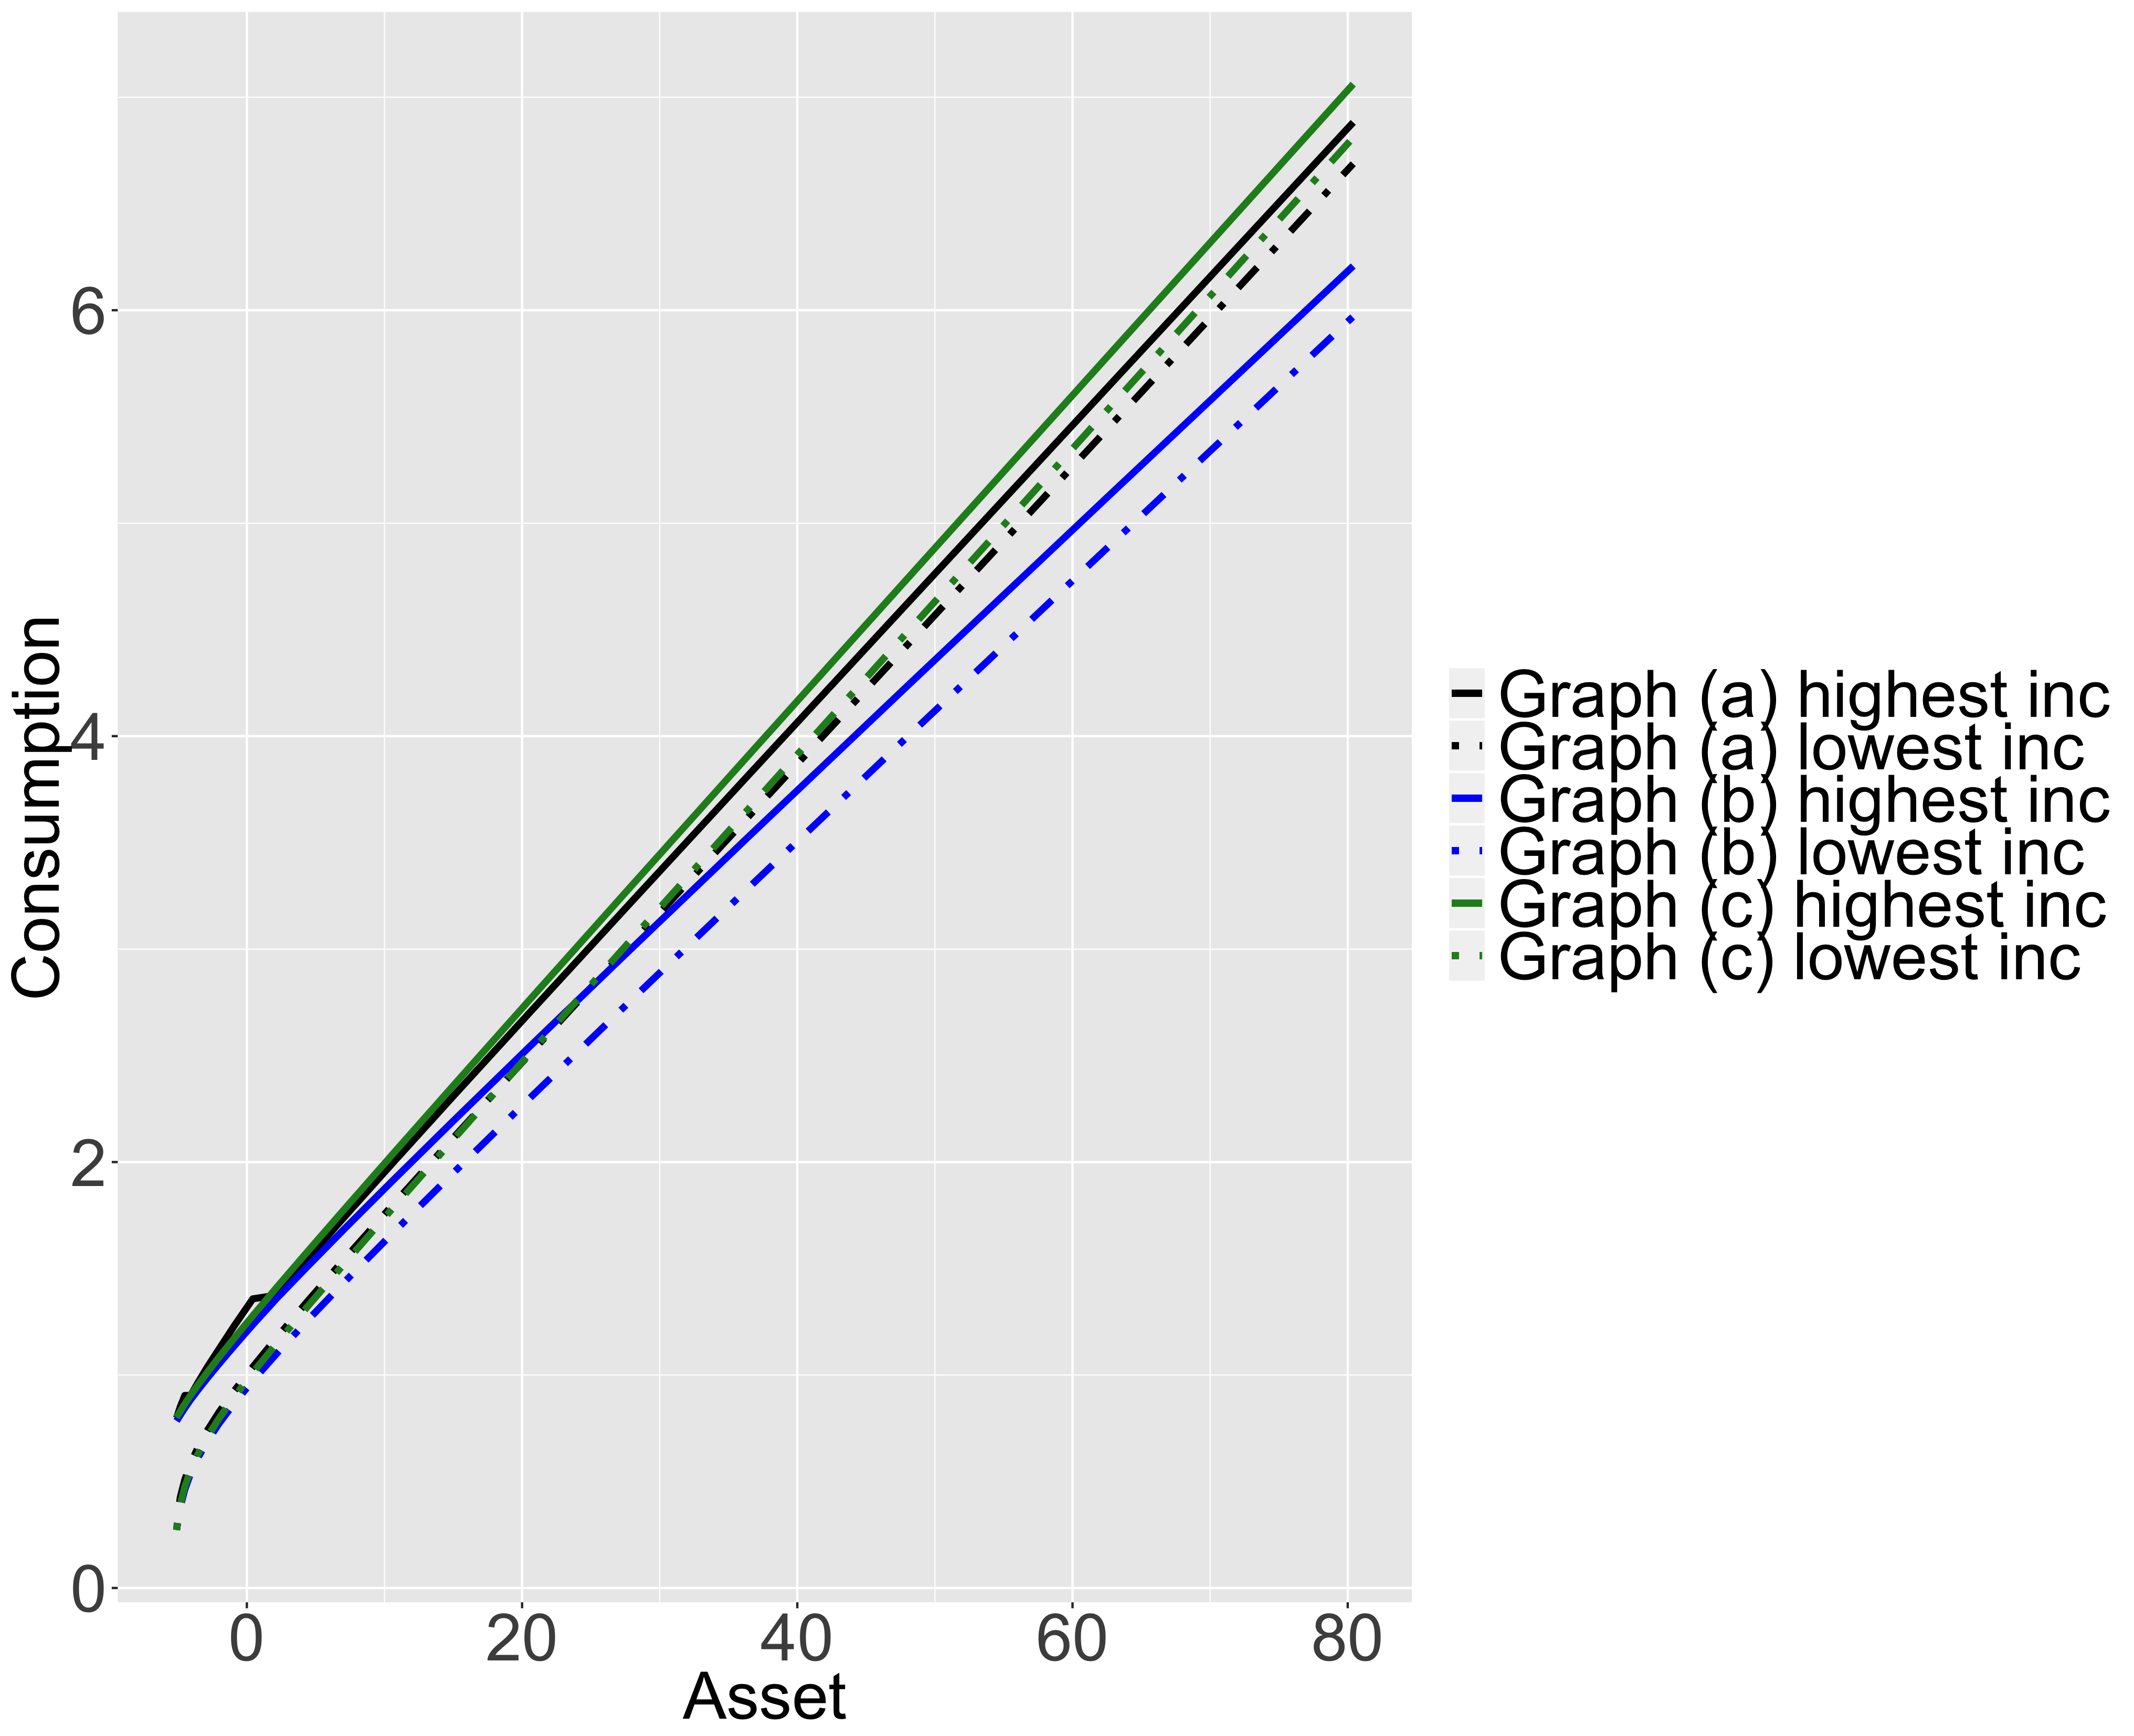
\includegraphics[width=0.8\linewidth]{Question2}
\label{fig:question2}
\end{figure}

We don't know analytical solution when income is uncertain, so we can't comment on the degree of numerical errors. However, the graph shows that different solution methods give slightly different policy functions, which can be attributed to differences in numerical errors. The solution method (a) and (c) give similar answers. The dotted line (corresponding to the lowest income) is always below the solid line (corresponding to the highest income), because the marginal propensity to consume is greater than zero. \\

\vspace{0.2in}
\textbf{Question 3. computing simulated moments on consumption and asset} \\
\begin{figure}[H]
\centering
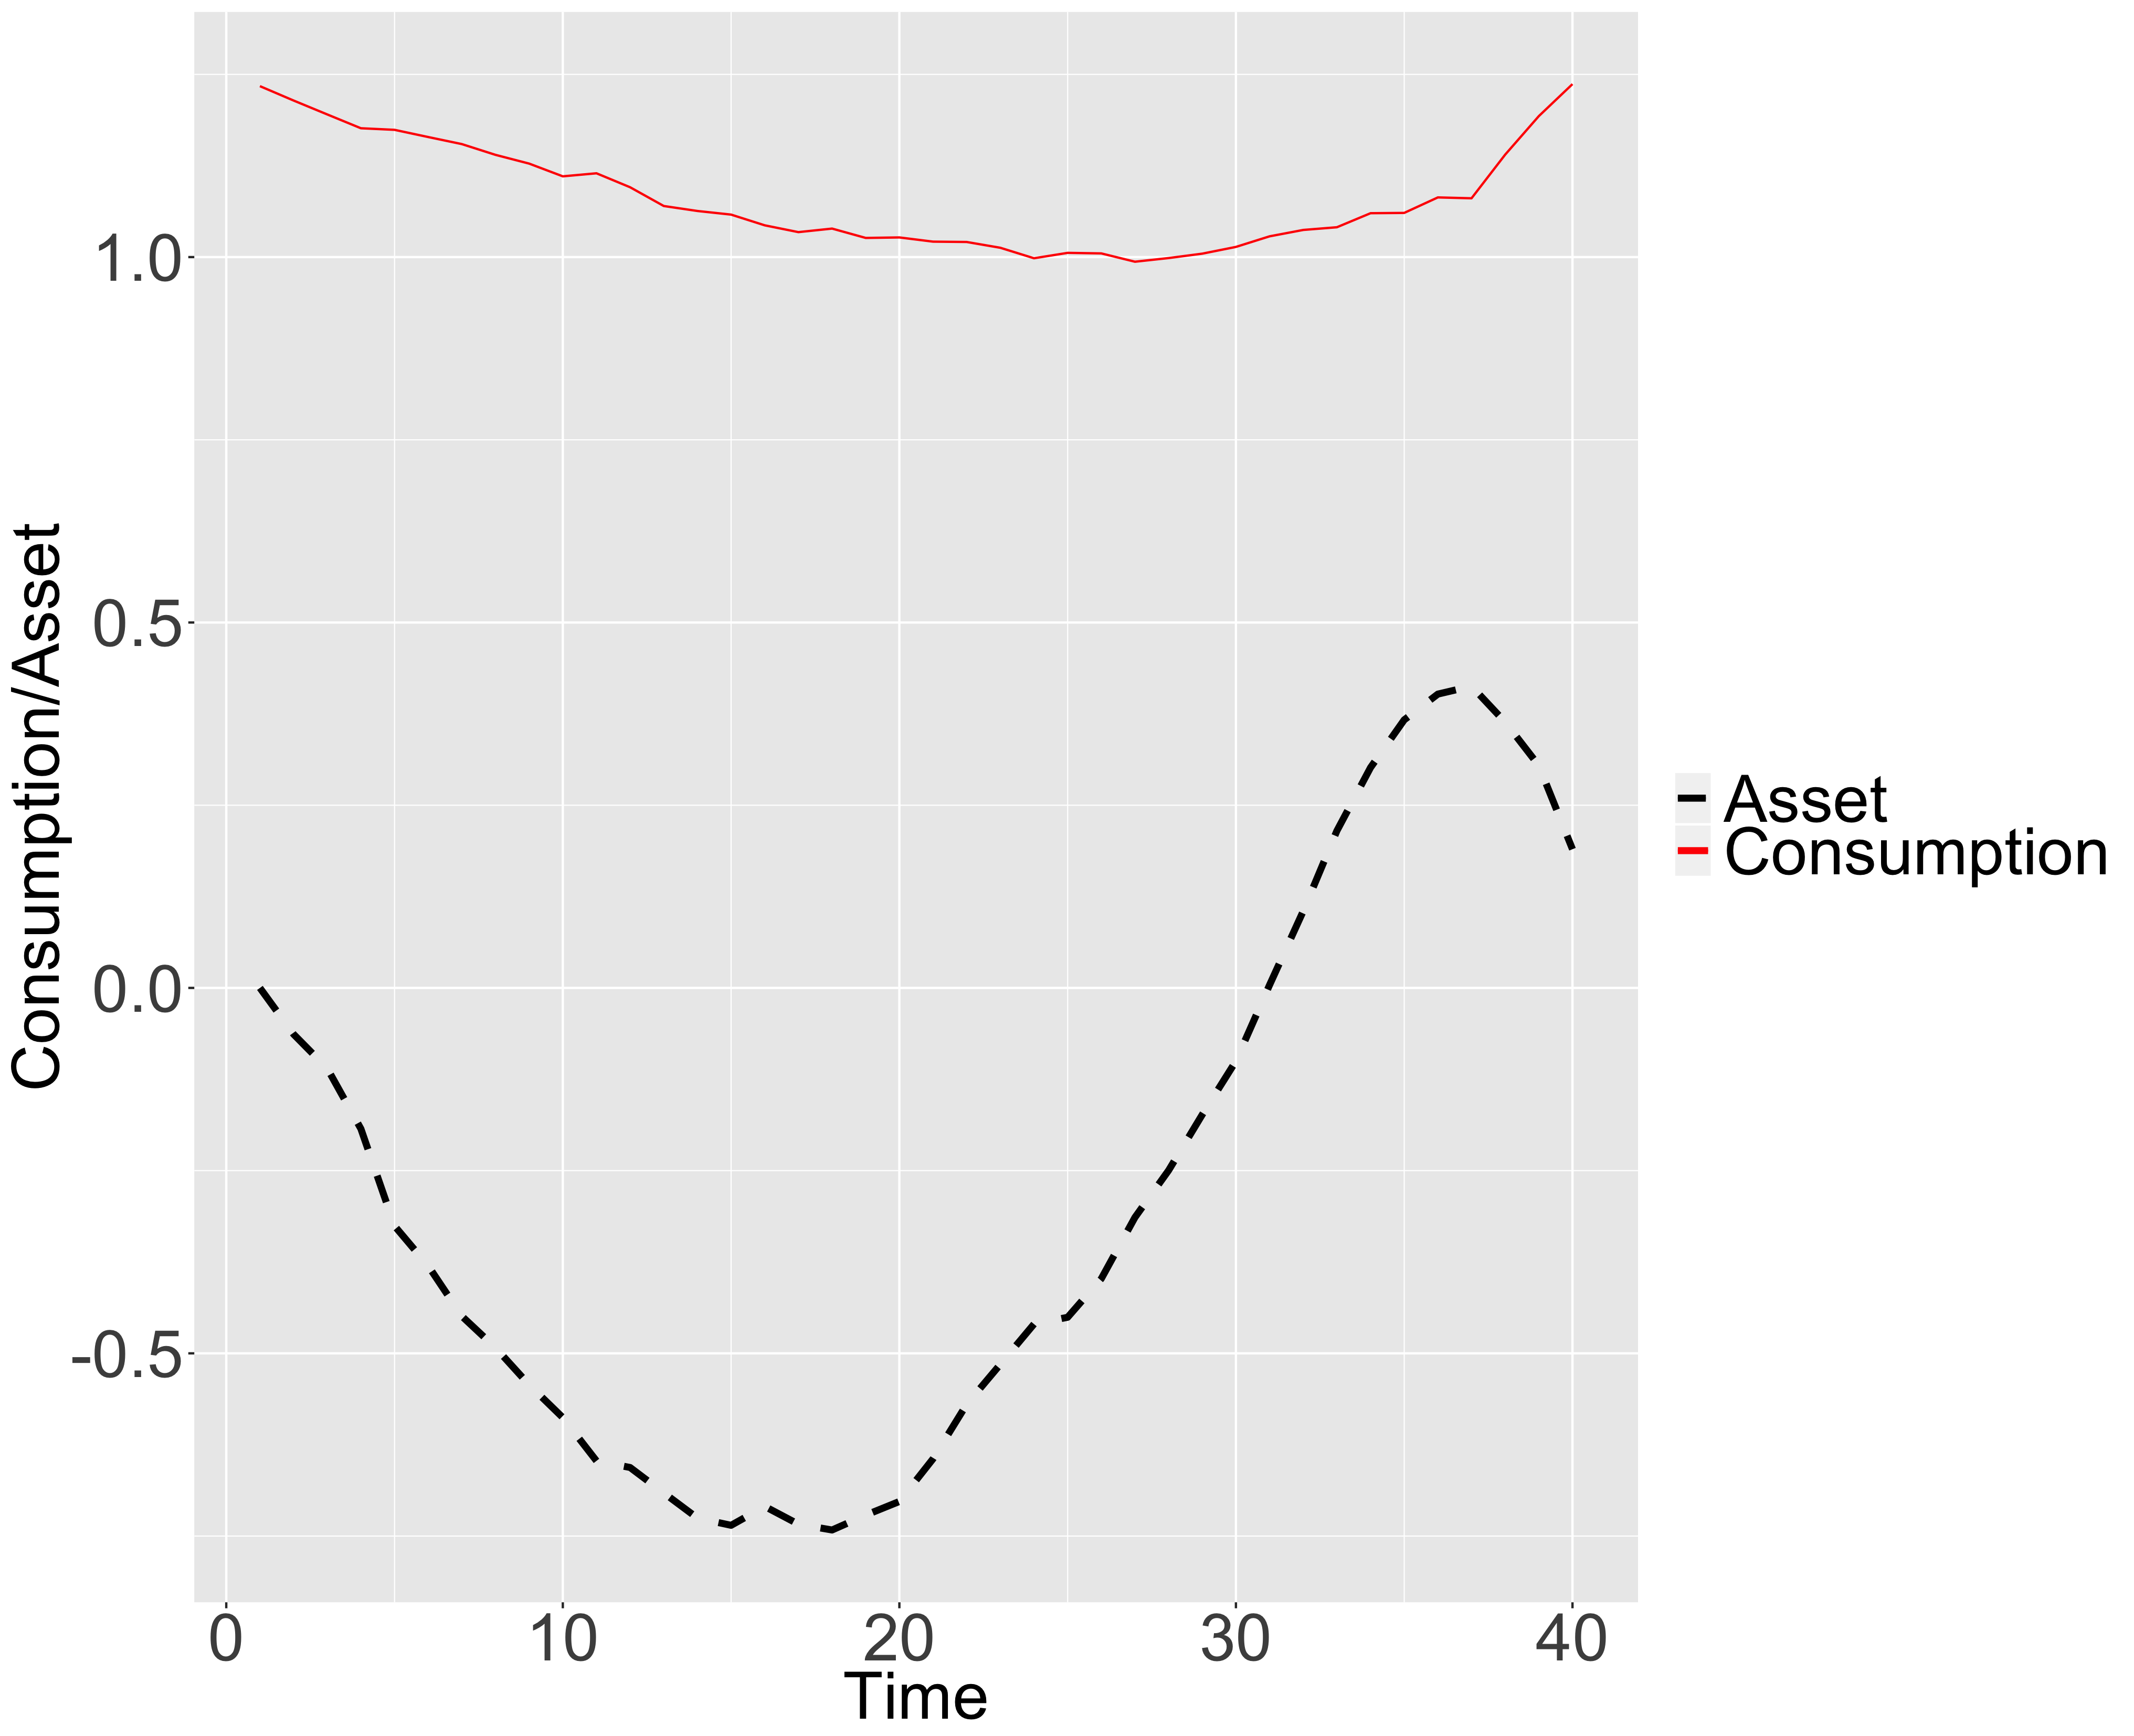
\includegraphics[width=0.7\linewidth]{Question3}
\label{fig:question3}
\end{figure}

Note that $\beta (1+r) =0.978 \leq 1$. Therefore, it is better for the agent to borrow heavily when young. As the agent gets older, the agent accumulates more assets to avoid default before death. In the last lifetime period, the agent consumes everything on hand. \\

\end{document}